%% All Observations
\subsection{Summary Stat for all Obs}
\begin{figure}[h]
    \centering
    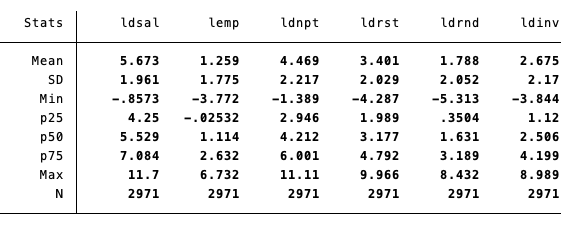
\includegraphics[height=5cm]{HW1/LATEX/Attachments/q1_stat_all.png}
    \caption{Summary Stat for all Obs}
    \label{fig:my_label}
\end{figure}

\begin{figure}[h]
    \centering
    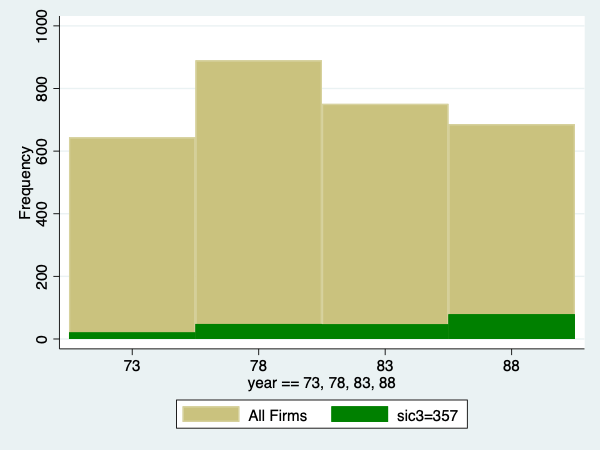
\includegraphics[height=6cm]{HW1/LATEX/Attachments/q1_all.png}
    \caption{Number of All Firms and SIC3=357}
    \label{fig:my_label}
\end{figure}

\newpage
%% Observations With at least 2 years
\subsection{Summary Stat for Obs with at lease 2 Year}
\begin{figure}[h]
    \centering
    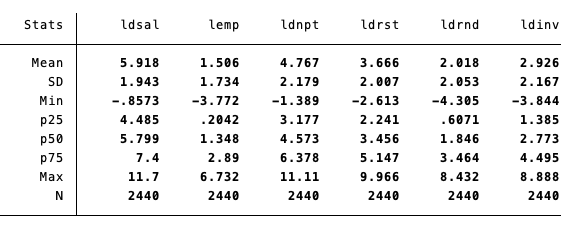
\includegraphics[height=7cm]{HW1/LATEX/Attachments/q1_stat_2.png}
    \caption{Summary Stat for Obs with at lease 2 Year}
    \label{fig:my_label}
\end{figure}

\begin{figure}[h]
    \centering
    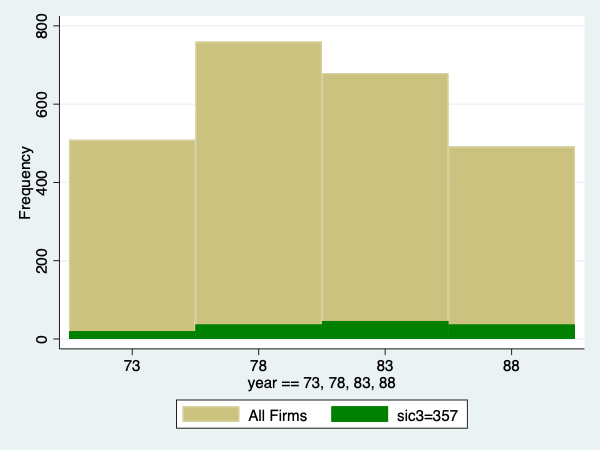
\includegraphics[height=9cm]{HW1/LATEX/Attachments/q1_2.png}
    \caption{Number of All Firms and SIC3=357 with at lease 2 Year}
    \label{fig:my_label}
\end{figure}

\newpage
%% Observations of balanced panel
\subsection{Summary Stat for Balanced Panel}
\begin{figure}[h]
    \centering
    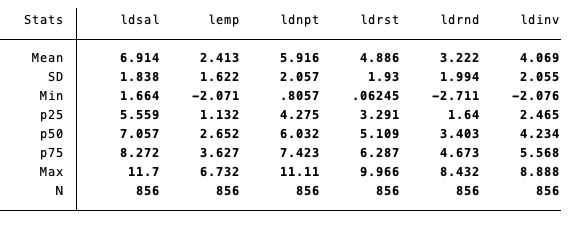
\includegraphics[height=7cm]{HW1/LATEX/Attachments/q1_stat_balanced.png}
    \caption{Summary Stat for Balanced Panel}
    \label{fig:my_label}
\end{figure}

\begin{figure}[h]
    \centering
    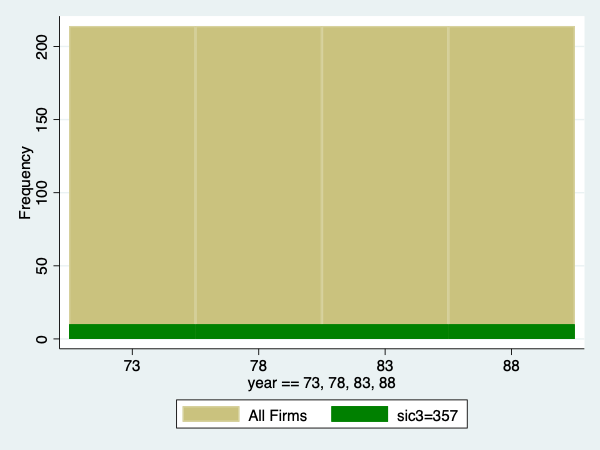
\includegraphics[height=9cm]{HW1/LATEX/Attachments/q1_balanced.png}
    \caption{Number of All Firms and SIC3=357 in Balanced Panel}
    \label{fig:my_label}
\end{figure}



\subsection{What does it suggest?}
As we can see, summary stat of data is changing. Fas we move from the total sample to the balanced sub-panel, the means of all the variables increase, while the standard deviations decrease. This may reflect sample selection: larger firms are more likely to survive for longer period.